\section{Deployment view (UML Deployment diagram)}\label{sec:deployment}

\begin{sidewaysfigure}[!htp]
    \centering
    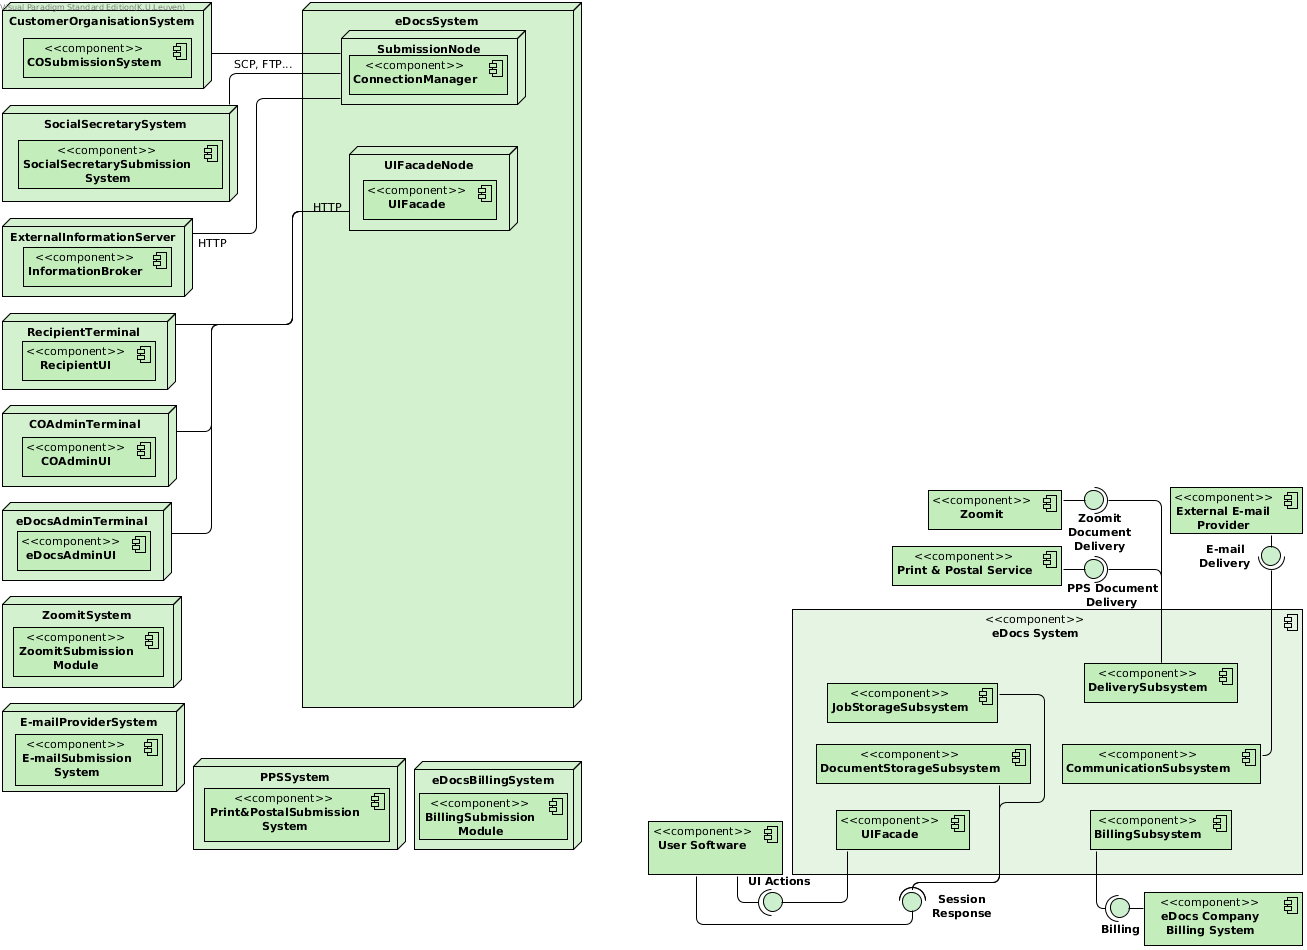
\includegraphics[width=0.8\textwidth]{figures/Deployment Context.png}
    \caption{Context diagram for the deployment view.}\label{fig:depl_context}
\end{sidewaysfigure}

Figure \ref{fig:depl_context} shows the Context Diagram for the deployment of the system.\\
The \ttt{SubmissionSubsystem} is contacted for Raw Data Submission over FTP, SCP, etc. as stipulated in the SLA (conform the initial description). The \ttt{Subsystem} also connects to an \ttt{InformationBroker} over HTTP to lookup information for consistency checks of Raw Data.\\
The different types of UIs (the \ttt{RecipientUI}, \ttt{COAdminUI} and \ttt{eDocsAdminUI}) connect to the UIFacade through the HTTP protocol, be it via a web browser or a user application. The response from a user's session is delivered back by the UIFacade (more precisely by the session of the user on the serverside) over the same protocol.\\
The \ttt{DeliveryChannels} send documents to their respective services over the protocol as stipulated by the service (FTP,SCP,...).\\
Nodes from the \ttt{CommunicationSubsystem} use SMTP to send e-mails via the \ttt{E-mailSubmissionSystem}, and the \ttt{ExternalNotificationAcceptor} also receives messages over SMTP from e.g. Zoomit or the e-mail provider (in case of failures, deliveries...).\\
The \ttt{BillingSubsystem} interfaces with an external billing system of the eDocs company through a general (FTP,SCP...) protocol to process billing to Customer Organisations.\\

\begin{sidewaysfigure}[!htp]
    \centering
    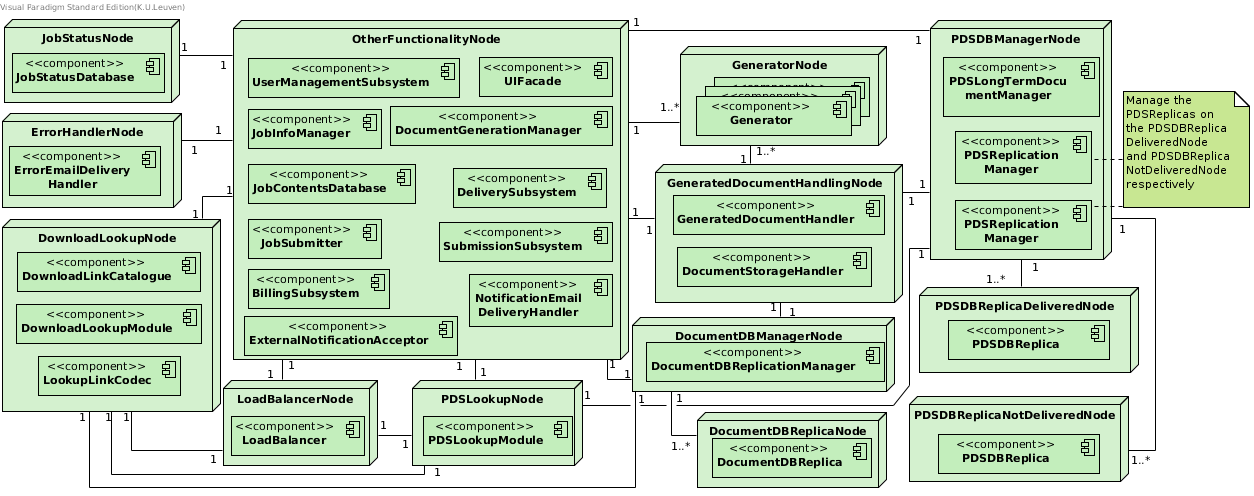
\includegraphics[width=0.9\textwidth]{figures/Deployment.png}
    \caption{Primary diagram for the deployment view.}\label{fig:depl_primary}
\end{sidewaysfigure}


\noindent Figure \ref{fig:depl_primary} presents the primary deployment of the internal architecture. All components for which no special deployment requirements were found are deployed on a general \ttt{OtherFunctionalityNode}.\\
The \ttt{Generator}s are deployed on dedicated \ttt{GeneratorNode}s as given initially. These connect to the \ttt{GeneratedDocumentHandler}, deployed on its own dedicated node. The reason for this being that this \ttt{Handler} can be a bottleneck in the system, since all generated documents pass through it. This way, a powerful node can be instated for this function, so it does not slow down the finalization of documents by the \ttt{Generator}s (\emph{P1}).\\
The \ttt{GeneratedDocumentHandlerNode} connects back to the \ttt{OtherFunctionalityNode} for delivery purposes, but the \ttt{DocumentStorageHandler} component on it also connects to both \ttt{DBManagerNode}s for storage purposes. This \ttt{DocumentStorageHandler} is hosted on the same node as the \ttt{GeneratedDocumentHandler} to lower the layers of indirection and boost performance.\\
The setup of the \ttt{PDSDB} nodes is the same as initially given, with the \ttt{PDSDBManagerNode} connecting to the \ttt{OtherFunctionalityNode} for various purposes, e.g. reporting \ttt{PDSDBReplica} failures.
Analogous to the \ttt{PDSDB}, the \ttt{DocumentDB} is deployed as a \ttt{DocumentDBManagerNode} and multiple \ttt{DocumentDBReplicaNode}s. This setup conforms to the active replication we set up for \emph{Av2} (e.g. filling the \ttt{PDSDB} after coming back online warrants a decent replication of the \ttt{DocumentDB}), but most importantly for performance sake by the use of sharding, for e.g. the aforementioned filling of the pds, while also storing new documents and simultaneously serving lookup requests (\emph{P2}).\\
Likewise, the components of the \ttt{LookupSubsystem} are deployed on their own respective nodes to suit \emph{P2} and connect to the necessary nodes for lookup. They are strongly interconnected, but have their own dedicated node, so load on one does not impact the other.\\
The \ttt{JobStatusDatabase} is deployed on its own node for \emph{P3}, being the single important component for this requirement.\\
The \ttt{ErrorEmailDeliveryHandler} is also deployed individually, playing a crucial role in \emph{Av1a} and \emph{Av2a}.

\subsection*{Alternatives Considered}
\paragraph{Not deploying the \ttt{ErrorEmailDeliveryHandler} on its own node} The \ttt{ErrorEmailDeliveryHandler} is not a very prominent component in the scenarios. An extra node means extra infrastructure, maintenance etc. On the other hand, not deploying an extra node might make the guarantee of notification under one minute harder to make.

\paragraph{Deploying the \ttt{GeneratedDocumentHandler} and \ttt{DocumentStorageHandler} on the \ttt{OtherFunctionalityNode}} The introduction of the \ttt{GeneratedDocumentHandlingNode} is not strictly necessary for \emph{P1}. We reasoned that since the \ttt{FinalizeDocument} operation is synchronous, eliminating a bottleneck in the generation flow would be advisable though. As mentioned, to adhere strictly to the non-functional requirements, we could also opt to deploy the components of the \ttt{GeneratedDocumentHandlingNode} on the \ttt{OtherFunctionalityNode}.

\paragraph{Deploying the \ttt{LookupSubsystem} on one dedicated \ttt{LookupNode}} The \ttt{LookupSubsystem} being deployed on multiple nodes makes them independantly robust, but due to the higher degree of indirection might negatively impact performance. If we deploy all components of the \ttt{LookupSubsystem} on a single node, performance goes up because of easier communication between e.g. the \ttt{LookupModules} and \ttt{LoadBalancer} or the \ttt{PDSLookupModule} and the \ttt{LookupLinkCodec}. However, this makes load on one \ttt{LookupModule} have a negative impact on the rest of the subsystem, being a performance tradeoff. Both options have their merit.